\documentclass{templatebeamerufc/libs/ufc_format}
% mini preambulo
\usepackage{subcaption} % subfigure, lado a lado
\usepackage{changepage} % ajusta margens do slide

% Insere preâmbulo com a importação de pacotes
\input{templatebeamerufc/libs/preamble.tex}
% Macros pessoais
%%% Local Variables:
%%% mode: latex
%%% TeX-master: t
%%% End:

% macros de utilidade
\newcommand{\fonteautor}{Elaborado pelo autor.}
\newcommand{\fonteautorscikit}{Elaborado pelo autor baseado nas
  imagens disponíveis em~\citeonline{scikit-image}.}
\newcommand{\red}[1]{\textcolor{red}{\textbf{#1}}}  % bold red text

\listfiles
% Título
\title[EGSIS]{\textbf{Segmentação Semi-Supervisionada de Imagens através de
Dinâmicas Coletivas em Redes Complexas}}
% Subtítulo
\subtitle{Um novo método avaliado no cenário de segmentação interativa}
% Autor da apresentação
\author[Manoel Vilela Machado Neto]{
  Manoel Vilela Machado Neto
  \\~\\
  Orientador: Dr.\ Jarbas Joaci de Mesquita Sá Junior
}
% Nome do instituto
\institute[UFC]{
    % email para contato
    \normalsize{\email{manoel.machado@alu.ufc.br}}
    \newline
    % Nome do departamento
    \department{Engenharia da Computação}
    \newline
    % Nome da universidade
    \ufc{}
}
% date of the presentation
\date{Sobral, 12 de dezembro de 2023}


%%%%%%%%%%%%%%%%%%%%%%%%%%%%%%%%%%%%%%%%%%%%%%%%%%%%%%%%%%%%%%%%%%%%%%%%%%%%%%%%%%
%% Inicío do Documento de Apresentação                                          %%
%%%%%%%%%%%%%%%%%%%%%%%%%%%%%%%%%%%%%%%%%%%%%%%%%%%%%%%%%%%%%%%%%%%%%%%%%%%%%%%%%%
\begin{document}
% Insere o estílo de código (quase não usado)
\input{templatebeamerufc/libs/code_style}
%% ---------------------------------------------------------------------------
% Primeiro slide (com título, subtítulo, ...)
\begin{frame}{}
    \maketitle
\end{frame}

%% ---------------------------------------------------------------------------
% Segundo slide com sumário
\begin{frame}[t, allowframebreaks]{Sumário}
  \tableofcontents[sections={1---2}]  % chktex 8
    \framebreak{}
  \tableofcontents[sections={3---6}]  % chktex 8
\end{frame}

%% ---------------------------------------------------------------------------------
%% ------------ INTRODUÇÃO -------------------------------
%% ---------------------------------------------------------------------------------
\section{Introdução}

%% ---------------------------------------------------------------------------
\subsection{Tipos de segmentação de imagem}

\begin{frame}{Segmentação de imagens}
  \begin{block}{Definição}
    Segmentar uma imagem significa dividí-la em regiões de interesse.
  \end{block}

  Existem alguns tipos diferentes de segmentação de imagens, como por
exemplo:
  \begin{enumerate}
    \item Segmentação semântica;
    \item Segmentação de instâncias;
    \item Segmentação interativa.
  \end{enumerate}
\end{frame}


\begin{frame}{Segmentação de instâncias e semântica}
  % imagem comparando segmentação semântica vs segmentação por instâncias
  \begin{figure}\label{fig:semantic-vs-instance-segmentation}
    \centering
    \caption{Comparação entre segmentação semântica e segmentação de instâncias.}
    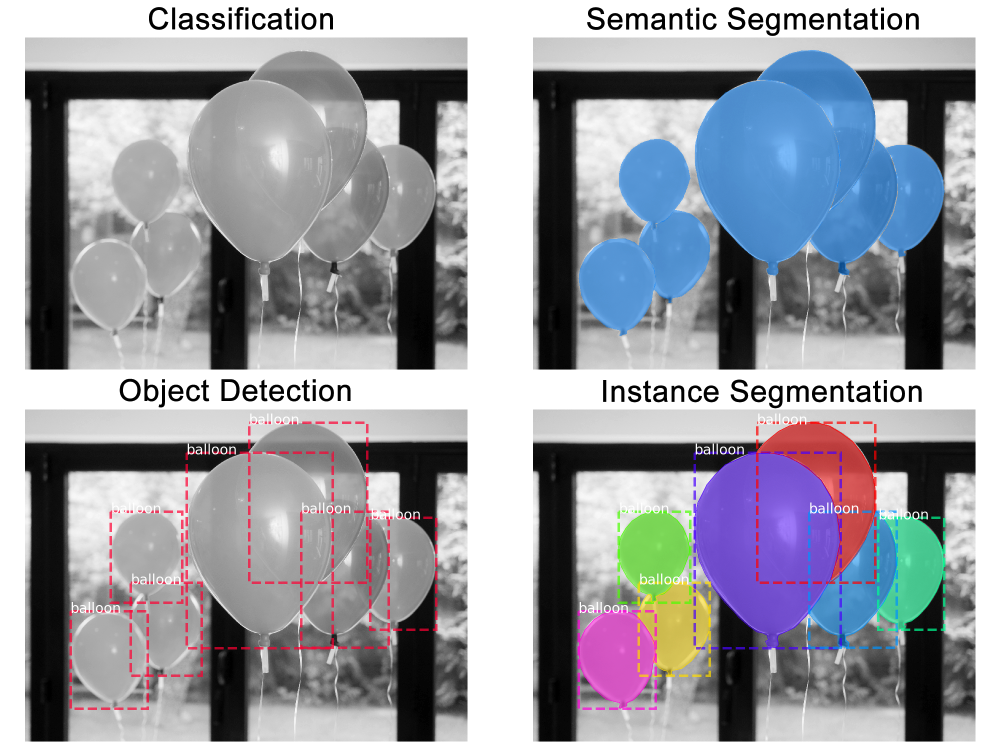
\includegraphics[scale=0.23]{figuras/image-segmentation-types}
    \source{\cite{MediumInstanceSegmentation2019}}
  \end{figure}
\end{frame}

\begin{frame}{Segmentação interativa}
  \begin{figure}\label{fig:interactive--segmentation}
    \centering
    \caption{Ilustração de segmentação interativa, rotulações em azul  e
      vermelho.\\ Na imagem à direita, após segmentação o fundo foi removido.}
    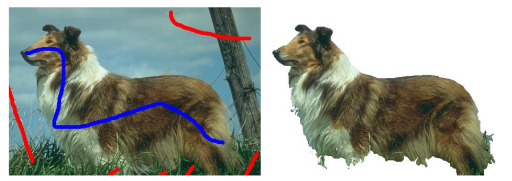
\includegraphics[scale=0.6]{figuras/interactive-segmentation-2008}
    \source{\cite{duchenne2008segmentation}}
  \end{figure}
\end{frame}

\begin{frame}{Segmentação interativa: alguns casos de uso}
  \begin{enumerate}
  \item \textbf{Medicina}: usada para identificar e isolar áreas específicas de
    interesse em imagens médicas, como tumores em imagens de
    ressonância magnética ou células específicas em uma imagem de
    microscópio.

  \item \textbf{Edição de imagens}: usada para separar objetos de interesse do fundo.

  \item \textbf{Agricultura e Geologia}: usada para identificar áreas específicas
em fotos aéreas ou de satélite para uso na agricultura de precisão e
estudos geológicos.
  \end{enumerate}
\end{frame}

%% ---------------------------------------------------------------------------
\subsection{Aprendizado de máquina}

\begin{frame}{Aprendizado de máquina}
  Em~\cite{samuel1959some}, aprendizado de maquina é definido como:

  \begin{block}{Definição} Campo de estudo que dá aos computadores a
    habilidade de aprender sem serem explicitamente programados.
  \end{block}

  \pause{}

  \begin{figure}\label{fig:samuel}
    \centering
    \caption{
      Arthur Samuel, 1956, apresenta sua criação ao público na
      TV, uma inteligência artificial capaz de jogar damas no
      computador IBM 701.
    }
    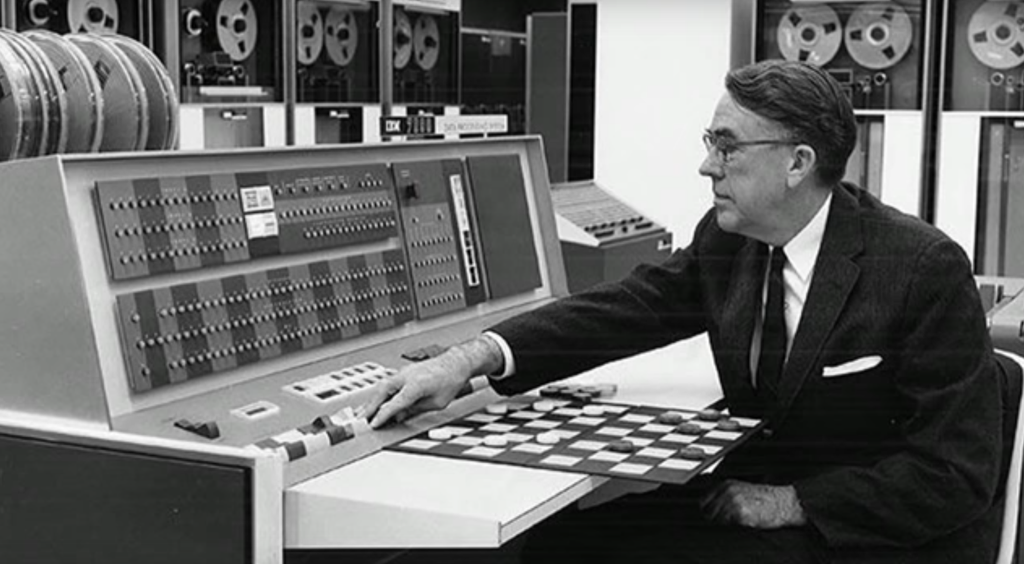
\includegraphics[scale=0.18]{figuras/samuel}
    \source{\cite{press2021machine}}
  \end{figure}
\end{frame}

\begin{frame}{Aprendizado semi-supervisionado}
  \begin{figure}\label{fig:ilustracao-aprendizado-semi-supervisionado}
    \centering
    \caption{
      O aprendizado semi-supervisionado tem como principal
característica \\ a utilização de dados rotulados e não rotulados na base
de treinamento.
}
    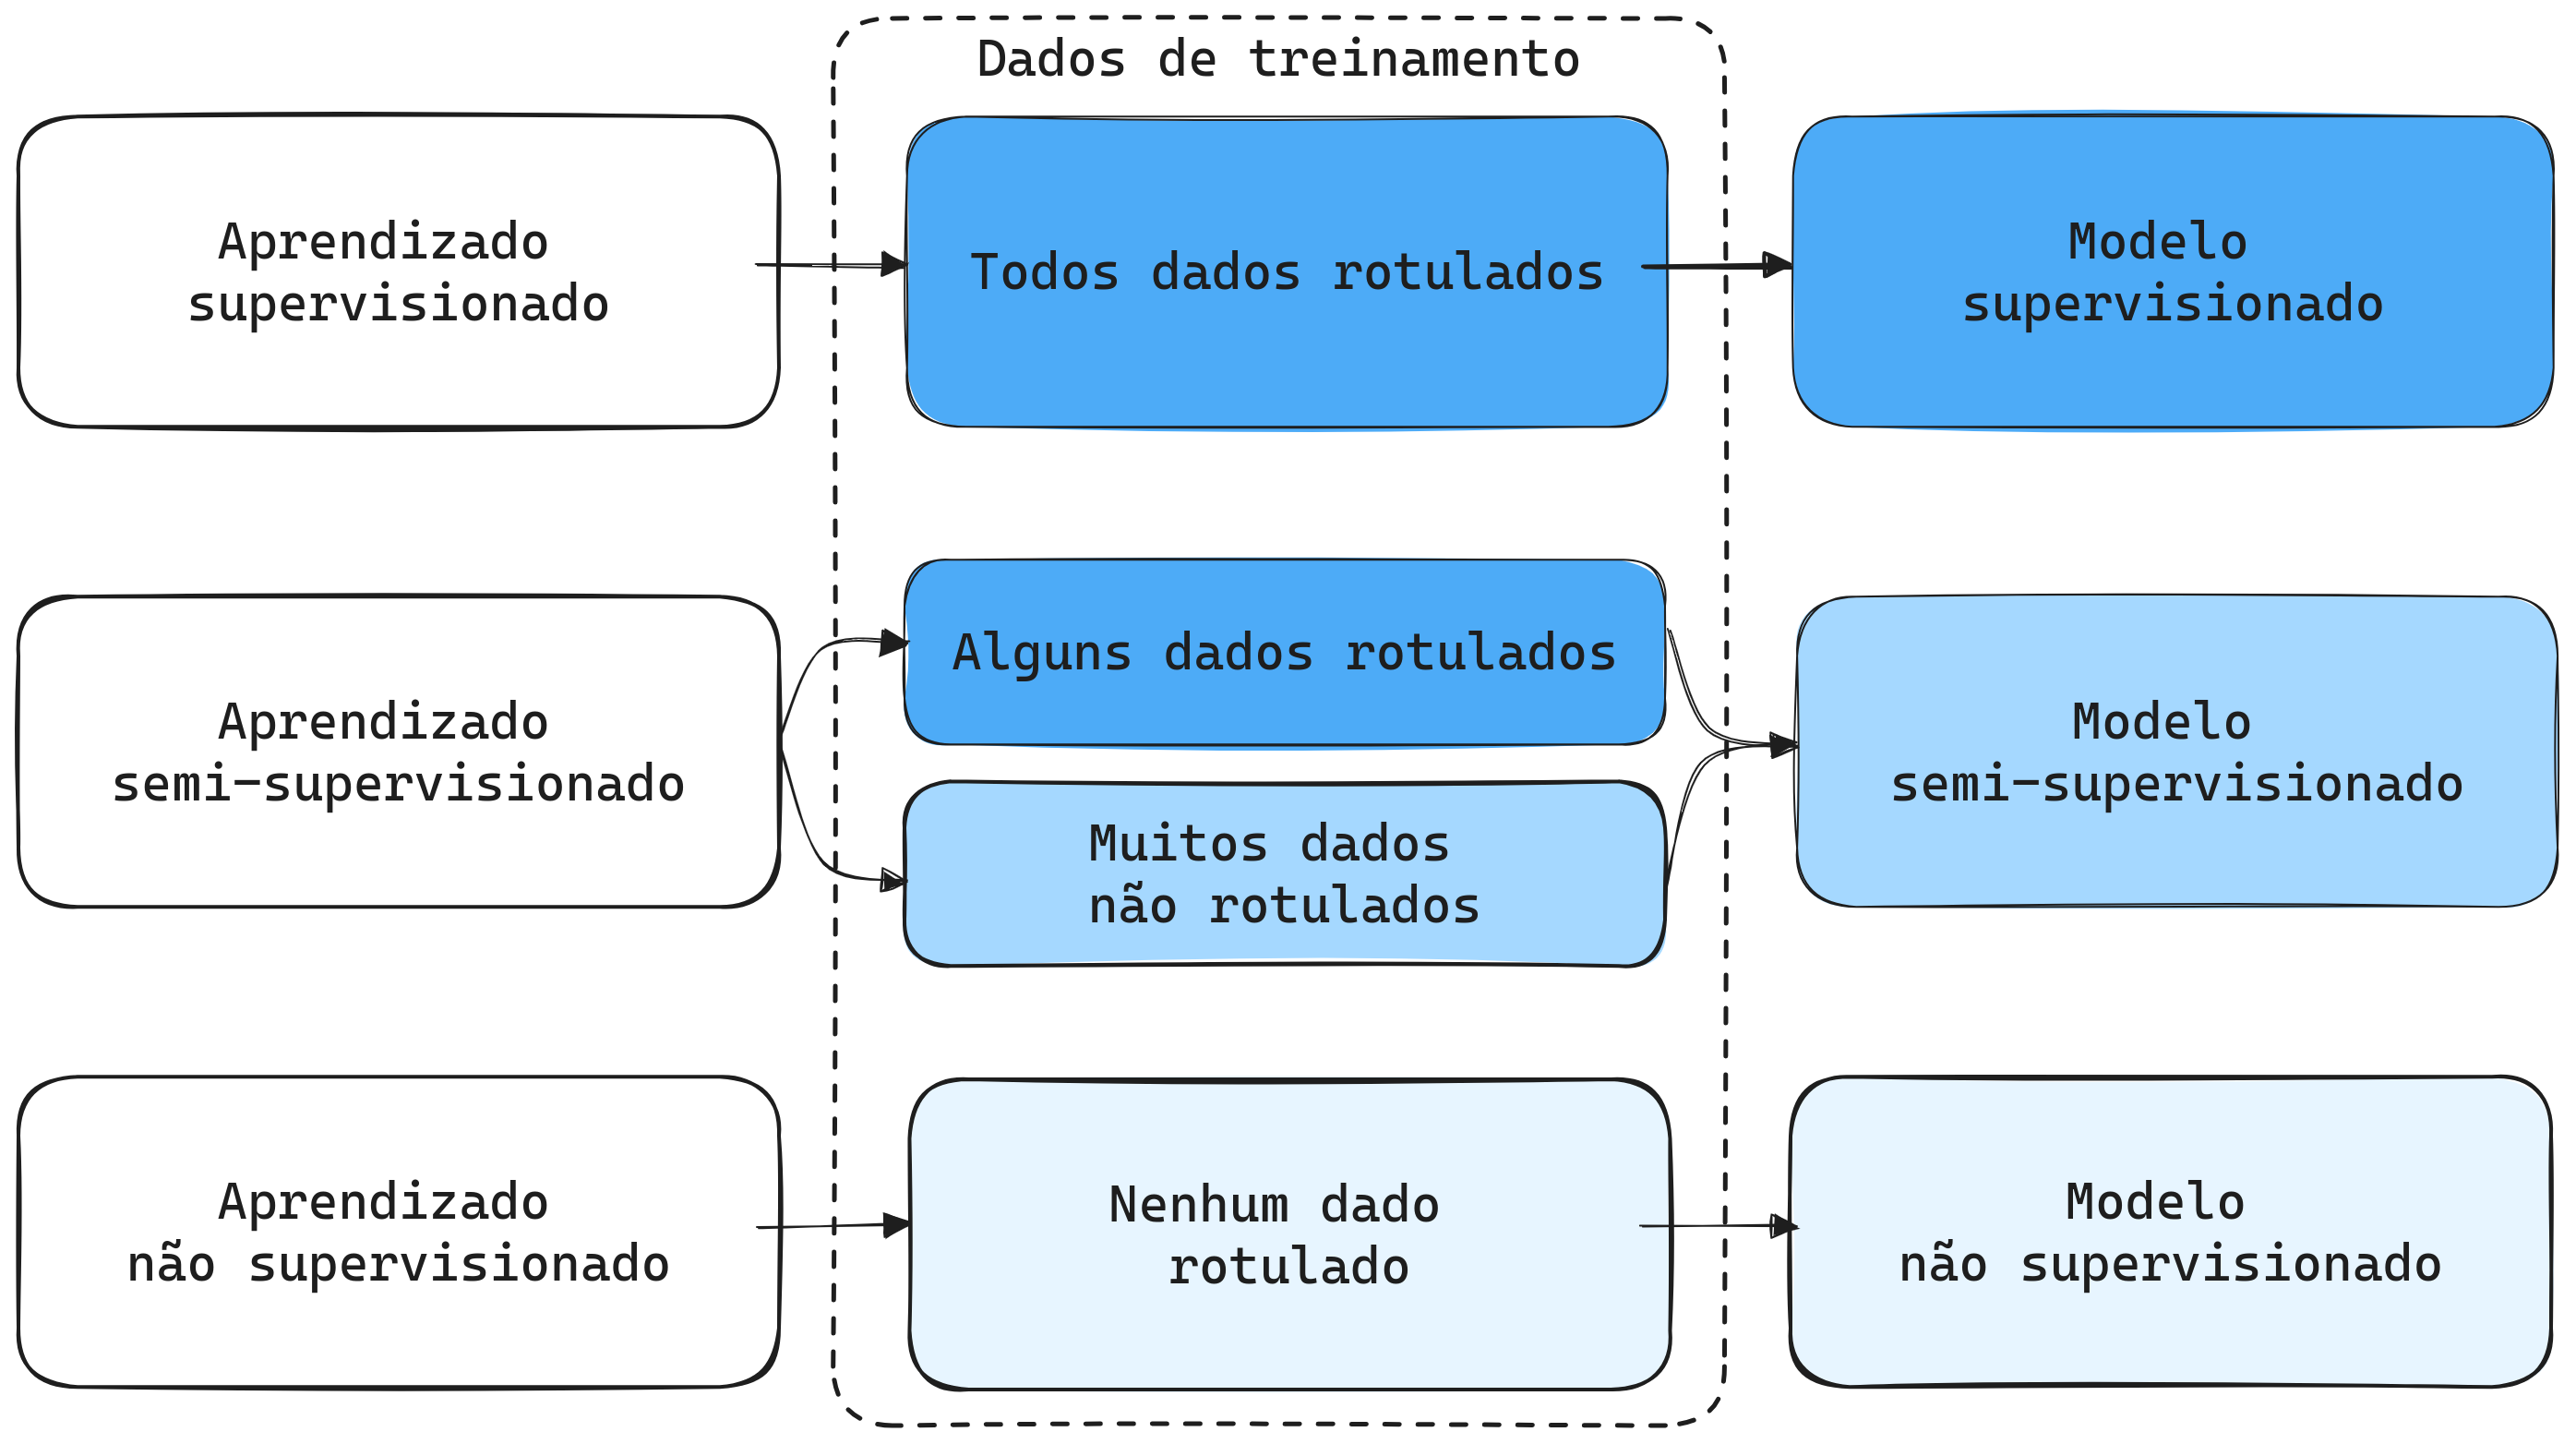
\includegraphics[scale=0.1]{figuras/ilustracao-aprendizado-semi-supervisionado}
    \source{\fonteautor}
  \end{figure}
\end{frame}


\begin{frame}{Aprendizado semi-supervisionado}
  \begin{block}{Dados de treinamento}
    Dado um conjunto de dados de treinamento $ \mathbf{X} =
    \{\vec{x_1}, \vec{x_2}, \ldots, \vec{x_n}\} $, tal que $ \vec{x_n} \in \mathbb{R}^d $,
    apenas um subconjunto $ \vec{Y} = \{y_1, y_2, \ldots , y_m\} $,
    em que $ (m < n) $, tem rótulos correspondentes.
  \end{block}

  \pause{}

  \begin{block}{Objetivo}
    O objetivo do aprendizado semi-supervisionado é usar tanto o
conjunto de dados rotulado quanto o não rotulado para aprender a
função $ f: \mathbf{X} \rightarrow \vec{Y} $ que pode prever o rótulo $ y $ para
um novo exemplo $ \vec{x} $.
  \end{block}
\end{frame}


\subsection{Aprendizado indutivo vs aprendizado transdutivo}

\begin{frame}{Aprendizado indutivo vs aprendizado transdutivo}
  \begin{figure}\label{fig:induction-vs-transudciton-cropped}
    \centering
    \caption{
      No aprendizado indutivo, como em redes neurais, uma função de
inferência é estimada durante o treinamento. Enquanto isso,
no aprendizado transdutivo a inferência de novos pontos é realizado sem a
necessidade de estimar essa função.
}
    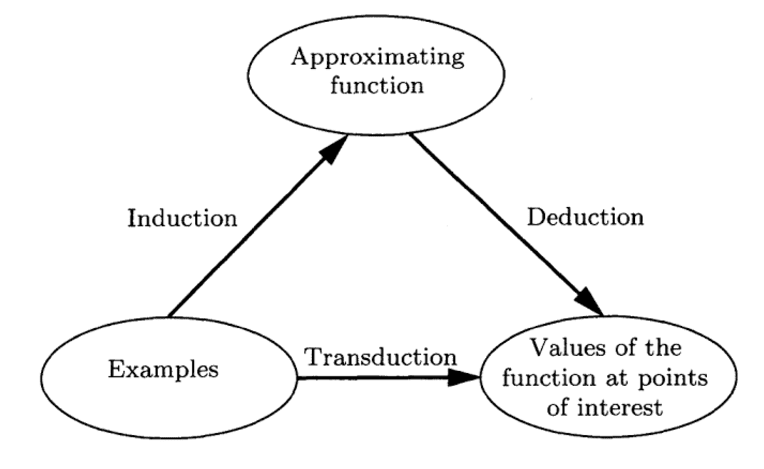
\includegraphics[scale=0.42]{figuras/induction_vs_transduction_cropped}
    \source{\cite{vapnik1995}}
  \end{figure}
\end{frame}

\begin{frame}{Aprendizado indutivo vs aprendizado transdutivo}
  \begin{figure}\label{fig:transductive-vs-inductive}
    \centering
    \caption{ Uma ilustração de aprendizado indutivo e aprendizado
      transdutivo.  }
    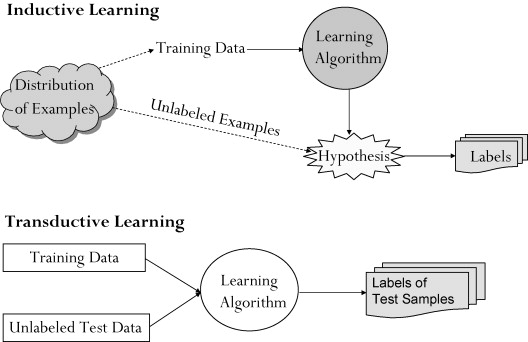
\includegraphics[scale=0.75]{figuras/transductive-vs-inductive}
    \source{\cite{vapnik1995}}
  \end{figure}
\end{frame}


\subsection{Objetivos}
\begin{frame}{Objetivos}
  \begin{alertblock}{Objetivo Geral}
    Desenvolver uma nova técnica de segmentação de imagens
    semi-supervisionada que possa ser equiparável ao estado-da-arte, com
    foco em \textbf{segmentação interativa}.
  \end{alertblock}
  \pause{}
  \begin{itemize}[<+->]
  \item Explorar técnicas de redes complexas e dinâmicas coletivas sobre
    o problema de segmentação de imagens;
  \item Aplicar em casos variados de segmentação de imagens, como
    objetos comuns, carros, pessoas, etc.;
  \item Avaliar o impacto da segmentação por superpixel na segmentação final;
  \end{itemize}

\end{frame}


%% -----------------------------------------------------------------------------------
%% ----- FUNDAMENTAÇÃO TEÓRICA ---------
%% ------------------------------------------------------------------------------------
\section{Fundamentação Teórica}
\subsection{Superpixels}
\begin{frame}{Superpixels}
  \begin{columns}{}

    \begin{column}{0.6\textwidth}
      \begin{block}{Definição}
        Superpixels são parte de um grupo de algoritmos de
        \textbf{clusterização} de imagens.
      \end{block}

      \begin{itemize}
      \item Eles agrupam pixels vizinhos semelhantes em uma entidade
        maior, conhecida como superpixel;
      \item Eles são formados com base na similaridade dos pixels em
        termos de cor, intensidade e localização na imagem.
      \end{itemize}
    \end{column}

    \begin{column}{0.5\textwidth}
      \begin{figure}\label{fig:superpixel-variation}
        \centering
        \caption{Uma mulher com imagem clusterizada por diferentes
          quantidades de superpixels.}
        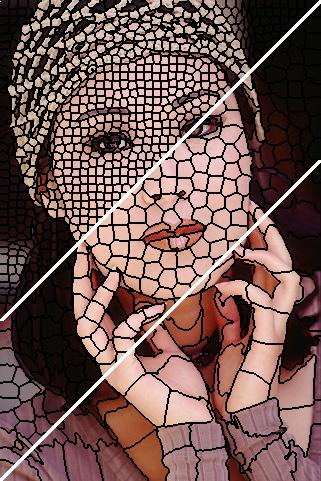
\includegraphics[scale=0.32]{figuras/superpixel-variation}
        \source{\cite{achanta2010slic}}
      \end{figure}n
    \end{column}
  \end{columns}
\end{frame}

\begin{frame}{Superpixels: SLIC}

  \begin{itemize}
  \item  O algoritmo SLIC~\cite{achanta2010slic} é um
    método para segmentação de imagens baseado em superpixel;
  \item Pode ser visto como uma variação do algoritmo de clusterização \textbf{k-means} expandindo
    o espaço euclidiano ao incluir também o espaço de cores.
  \end{itemize}
  \begin{figure}\label{fig:slic}
     \centering
        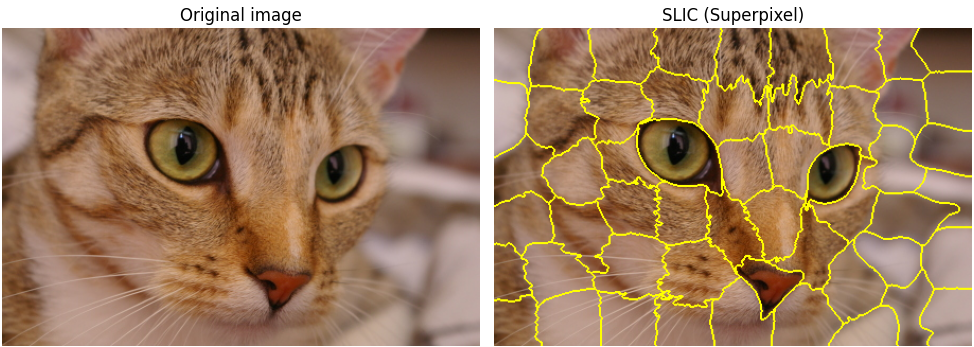
\includegraphics[scale=0.40]{figuras/slic2}
        \source{Elaborado pelo autor baseado em~\cite{scikit-image}.}
   \end{figure}
\end{frame}

\subsection{Redes complexas}

\begin{frame}{Redes complexas}
  \begin{block}{Definição}
    Redes complexas são grafos de topologia não-trivial.
  \end{block}
  \begin{itemize}
  \item Redes complexas são usadas para representar uma variedade de
sistemas e fenômenos em diversas áreas, incluindo física, biologia,
ciência da computação, engenharia e ciências sociais;
    \item Existem variados algoritmos para geração de redes complexas~\cite{ComplexNetworksSurvey2007};
    \item Redes complexas podem ser usadas como um domínio de dados para realizar várias tarefas, incluindo:
    \begin{enumerate}
        \item Classificação de imagens~\cite{ComplexNetworksImageClassification2015};
        \item Extração de características~\cite{JarbasComplexNetworks2020};
        \item Segmentação de imagens.
    \end{enumerate}
  \end{itemize}
\end{frame}

\begin{frame}{Geração de redes complexas}
  Neste trabalho, o uso de redes complexas é realizado de uma maneira
acoplada ao algoritmo de superpixels. Nesse cenário, cada superpixel
gerado na imagem é um \textbf{vértice} e as \textbf{arestas} são
geradas com base na vizinhança.

   \begin{figure}\label{fig:complex-networks-simplified}
     \centering
        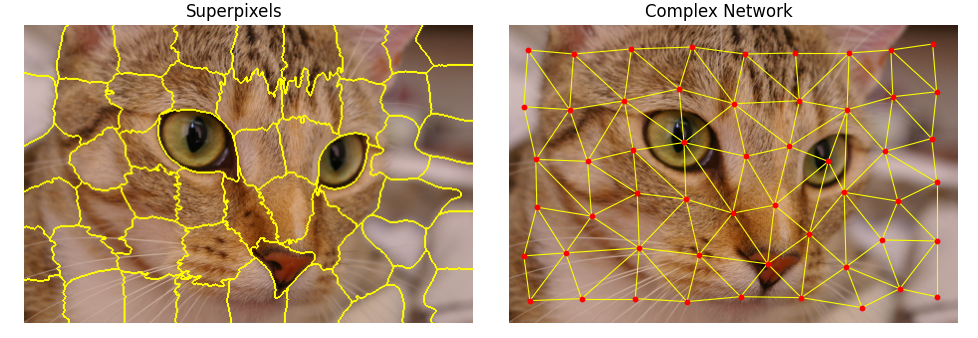
\includegraphics[scale=0.32]{figuras/complex-networks-simplified}
        \source{Elaborado pelo autor baseado em~\cite{scikit-image}.}
   \end{figure}
\end{frame}

\subsection{Extração de características}
\begin{frame}{Extração de características}
  \begin{itemize}
  \item A extração de características é realizada através de um
    \textbf{janelamento} na imagem pelo superpixel correspondente.
  \item Através de pequenos recortes retangulares e uma função de
extração de características, é calculado um vetor de características
que representa aquele \textbf{superpixel}.
  \end{itemize}

  \begin{figure}\label{fig:superpixels-feature-extraction}
    \centering
    \caption{Quatro superpixels recortados com o mesmo tamanho de janela.}
    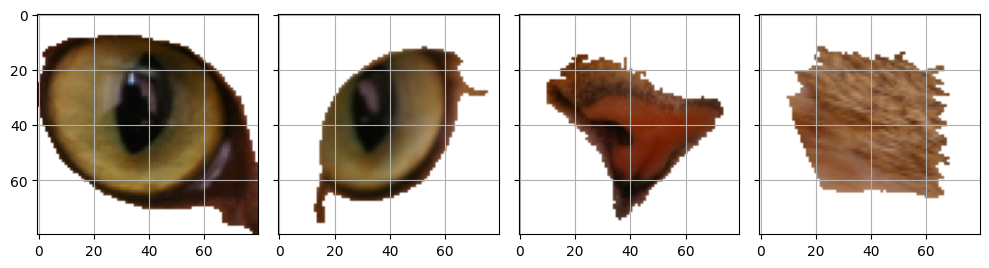
\includegraphics[scale=0.4]{figuras/superpixels-feature-extraction}
    \source{Elaborado pelo autor baseado em~\cite{scikit-image}.}
  \end{figure}

\end{frame}

\begin{frame}{Matriz de co-ocorrências}

  \begin{itemize}
  \item A matriz de co-ocorrências~\cite{haralick1979statistical} é uma técnica de processamento de
    imagem que extrai características de textura de uma imagem, contando a
    frequência de pares de pixels com intensidades específicas em
    distâncias definidas.
  \item A matriz é normalmente normalizada para se tornar uma matriz de
    probabilidade de co-ocorrência, a partir da qual características como
    contraste, correlação, energia e homogeneidade podem ser extraídas.
  \end{itemize}

  \begin{equation*}\label{eq:comatrix}
    C_{\Delta x, \Delta y}(i,j) = \sum_{x=1}^n\sum_{y=1}^m
    \begin{cases} 1, & \text{se }I(x,y)=i\text{ e }I(x+\Delta x, y+\Delta y)=j
      \\ 0, & \text{caso contrário}
    \end{cases}
  \end{equation*}

  Na equação acima, $C_{\Delta x, \Delta y}(i,j)$ é o número de vezes
  que o par de pixels com intensidades $i$ e $j$ ocorre em dois pixels
  separados pelas distâncias na imagem $I$.

  \vspace{1cm}
\end{frame}
\begin{frame}{Filtros de Gabor}
  \begin{block}{Definição simplificada}
      Os filtros de Gabor~\cite{daugman1988complete} são filtros de
convolução que podem ser usados na extração de características de
imagens.
  \end{block}
  \begin{figure}[!h]\label{fig:gabor-filters}
    \centering
    \caption{Filtros de Gabor variando a angulação $\theta$ e a convolução resultante.}
    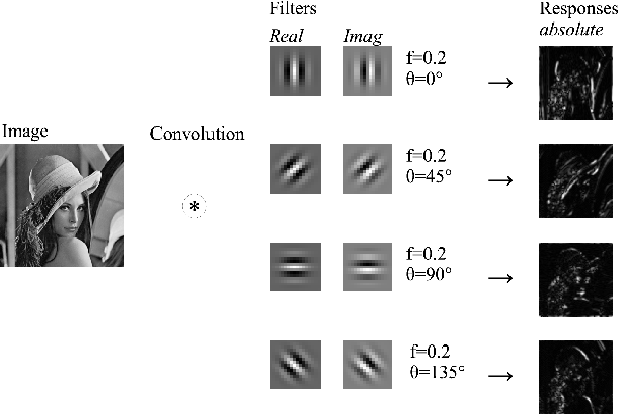
\includegraphics[scale=0.3]{figuras/gabor-filters}
    \source{\cite{Kmrinen2012GaborFI}}
  \end{figure}
\end{frame}

\subsection{Métricas de distância e similaridade}

\begin{frame}{Métricas de distância e similaridade}
\begin{itemize}
  \item Neste trabalho, as métricas de similaridade são utilizadas para comparar a
similaridade entre os vetores de características dos superpixels.
  \item Cada técnica de extração de características descrita nos
slides anteriores se comportou melhor com uma métrica de similaridade
diferente.
  \item Uma função de similaridade entre dois vetores de
características retorna um valor maior quando os vetores são similares
e tende a zero quanto mais são diferentes.
 \item O valor de similaridade determina o \textbf{peso da aresta} entre os dois superpixels.
\end{itemize}
\end{frame}

\begin{frame}{Métricas de distância}
  \begin{equation*}\label{eq:distancias}
    \begin{aligned}
      ed(\vec{x}, \vec{y}) &= \sqrt{{(y_1-x_1)}^2 + {(y_2-x_2)}^2 + \cdots + {(y_n-x_n)}^2} \\
      md(\vec{x}, \vec{y}) &= |y_1-x_1| + |y_2-x_2| + \cdots + |y_n-x_n|
    \end{aligned}
  \end{equation*}
  \begin{figure}[!h]
    \centering
    \caption{
      Este trabalho explora a criação de métricas de similaridade a
      partir de duas métricas de distância: a distância euclidiana e a
      distância de Manhattan.
    }
    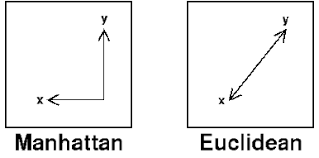
\includegraphics[scale=0.5]{figuras/manhattan-vs-euclidean}
    \source{\cite{Singh2019}}
  \end{figure}
\end{frame}

\begin{frame}{Métricas de similaridade}
  \begin{itemize}
  \item A distância euclidiana foi usada
    para formar a métrica de similaridade euclidiana exponencial, que se
    comportou melhor para \textbf{matrizes de co-ocorrências}.
   \item A distância de Manhattan foi usada para formar a métrica de
     similaridade de manhattan logarítmica, que se comportou melhor para
     \textbf{filtros de Gabor}.
  \end{itemize}

  \begin{equation*}\label{eq:similaridades}
    \begin{aligned}
      ed\_sim(\vec{x}, \vec{y}) &= \dfrac{1}{e^{ed(\vec{x}, \vec{y})}} \\
      md\_sim(\vec{x}, \vec{y}) &= \dfrac{1}{1 + \ln(1 + md(\vec{x}, \vec{y}))}
    \end{aligned}
  \end{equation*}

\end{frame}

\subsection{Dinâmicas coletivas}
\begin{frame}{Dinâmicas Coletivas}
  \begin{block}{Definição}
    Dinâmicas coletivas em redes complexas referem-se ao estudo de
como os comportamentos individuais interagem e se combinam para formar
comportamentos coletivos em redes.
  \end{block}
  \begin{enumerate}
\item Essas redes podem ser de vários tipos, como redes sociais, redes
de computadores, redes biológicas, entre outras.
\item Exemplos de dinâmicas coletivas:
  \begin{enumerate}
  \item Propagação de doenças em redes de contato;
  \item Disseminação de informações ou rumores em redes sociais;
  \item Formação de opiniões em grupos sociais;
  \item Sincronização de relógios biológicos em redes de neurônios.
  \end{enumerate}
\end{enumerate}
\end{frame}
\begin{frame}{LCU:\@ Labeled Component Unfolding}
  O algoritmo LCU~\cite{VerriNetworkUnfoldingMap2018} é uma dinâmica coletiva baseada em
propagação de rótulos numa rede complexa inspirada em fenômenos
naturais, como competição e sobrevivência.

\begin{figure}[!h]
\centering
    \caption{\label{fig:lcu-execution}
      Rede complexa para execução da dinâmica LCU.\@
      Anotação parcial em~(\subref{fig:lcu-partial}) e resultado final em~(\subref{fig:lcu-done}).
    }

    \begin{subfigure}[b]{0.45\textwidth}
    \centering
    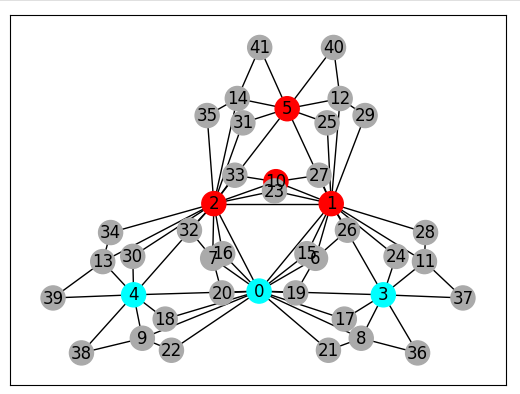
\includegraphics[scale=0.4]{figuras/lcu-partial}
    \caption{\label{fig:lcu-partial}}
    \end{subfigure}
\quad
    \begin{subfigure}[b]{0.45\textwidth}
    \centering
    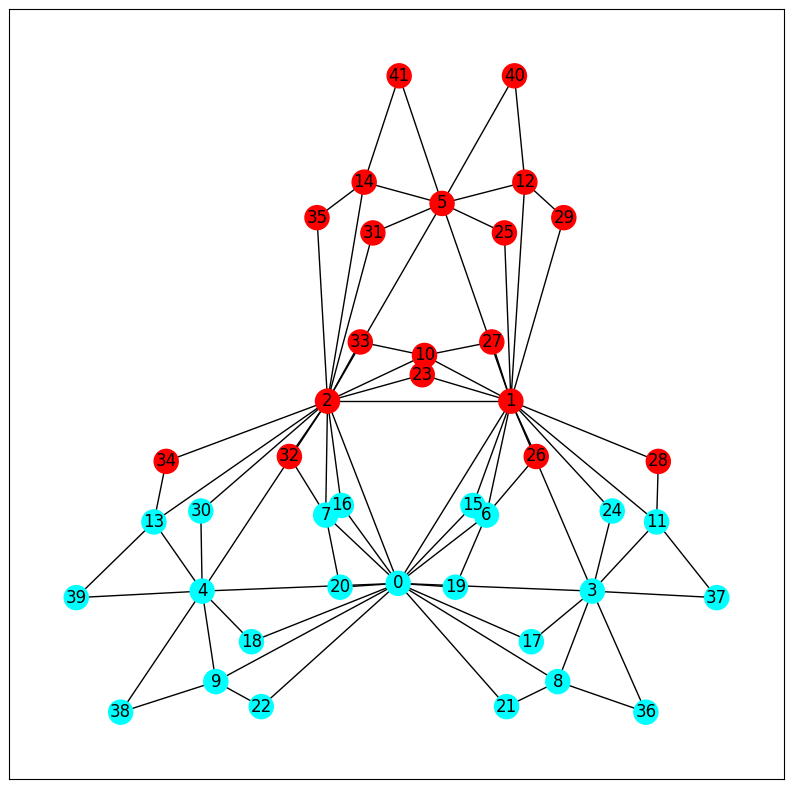
\includegraphics[scale=0.4]{figuras/lcu-done}
    \caption{\label{fig:lcu-done}}
    \end{subfigure}
    \source{\fonteautor}
\quad
\end{figure}
\end{frame}

\begin{frame}{LCU:\@ Labeled Component Unfolding}
  \begin{figure}[h!]\label{fig:lcu-classification-splig1}
    \centering
    \caption{
      Execução da dinâmica coletiva LCU:\@ (a) rotulação inicial nos
vértices e (b) algumas iterações com dominação de arestas.
    }
    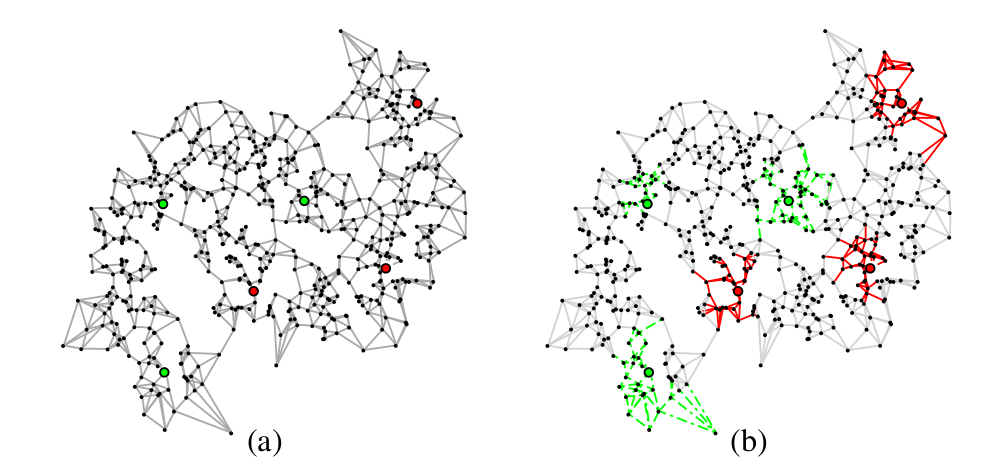
\includegraphics[scale=0.43]{figuras/lcu-classification-split1}
    \source{\cite{VerriNetworkUnfoldingMap2018}}
  \end{figure}
  \vspace{1cm}
\end{frame}

\begin{frame}{LCU:\@ Labeled Component Unfolding}
  \begin{figure}[h!]\label{fig:lcu-classification-split2}
    \centering
    \caption{
      Execução da dinâmica coletiva LCU:\@ (c) iteração avançada com
dominação completa das arestas e (d) propagação de rótulos nos vértices.
    }
    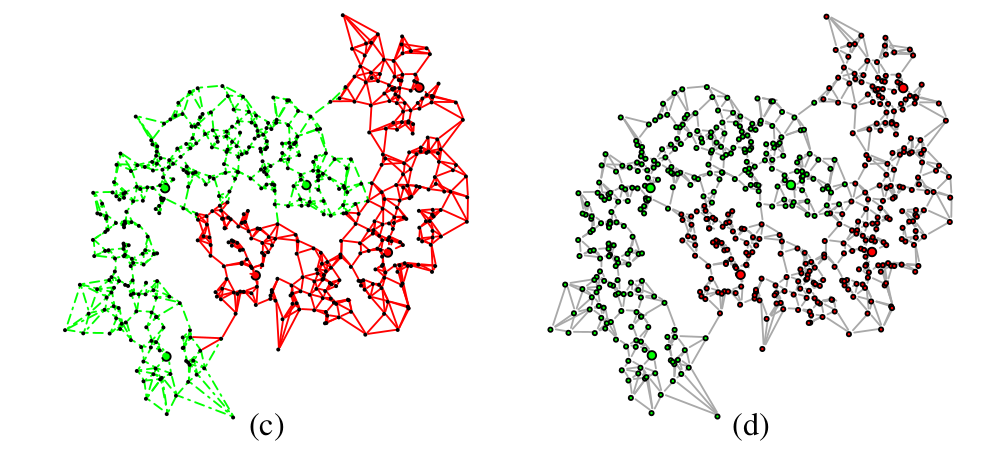
\includegraphics[scale=0.43]{figuras/lcu-classification-split2}
    \source{\cite{VerriNetworkUnfoldingMap2018}}
  \end{figure}

\end{frame}

\begin{frame}{LCU modificado com arestas ponderadas}
  \begin{columns}{}

    \begin{column}{0.6\textwidth}
      A implementação proposta neste trabalho difere da original,
      pois inclui a \textbf{similaridade de imagem} entre dois superpixels na rede
      complexa como \textbf{peso nas arestas}, criando um fator de aumento da
      probabilidade das partículas sobreviverem ao visitar os nós mais promissores.
    \end{column}

    \begin{column}{0.5\textwidth}
      \begin{figure}[h!]\label{fig:lcu-classification-split2}
        \centering
        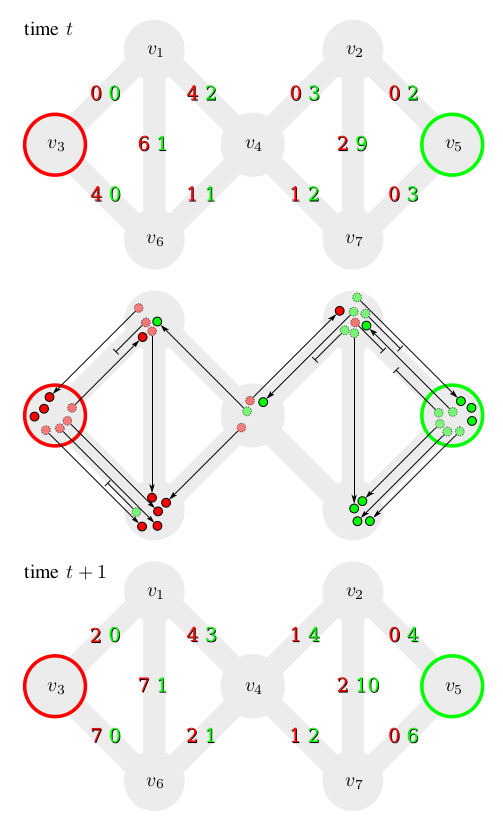
\includegraphics[scale=0.21]{figuras/lcu-iteration}
        \source{\cite{VerriNetworkUnfoldingMap2018}}
      \end{figure}
    \end{column}
  \end{columns}

\end{frame}
\subsection{EGSIS}

\begin{frame}{EGSIS}
  \textbf{E}xploratory \textbf{G}raph-based
  \textbf{S}emi-supervised \textbf{I}mage \textbf{S}egmentation (EGSIS) é
  a técnica de segmentação de imagens proposta proposta neste trabalho.

  \begin{enumerate}
  \item O modelo EGSIS permite a segmentação transdutiva de imagens
    na presença de uma rotulação parcial da imagem;
  \item Possui etapas flexíveis para refinamento e otimização,
    incluindo método de extração de características, quantidade de
    superpixels, função de similaridade, entre outros;
  \item O método de segmentação realiza uma transformação do domínio
    da imagem para uma rede complexa compatível com a dinâmica coletiva
    LCU.\@
  \end{enumerate}

\end{frame}

\begin{frame}{EGSIS:\@ Algoritmo}
  \begin{enumerate}
  \item Inicializa os hiperparâmetros do modelo EGSIS;\@
  \item Segmenta a imagem em $n$ superpixels usando SLIC;\@
  \item Realiza a construção da rede complexa baseado nos superpixels;
  \item Atribui os superpixels rotulados baseado na anotação parcial;
  \item Calcula o vetor de características para cada superpixel;
  \item Calcula a similaridade entre superpixels da vizinhança;
  \item Executa a dinâmica LCU sobre a rede complexa gerada;
  \item Reconstrói a máscara de segmentação com base nos vértices rotulados.
  \end{enumerate}
\end{frame}

%% -----------------------------------------------------------------------------------
%% ---------- METODOLOGIA ------------------------------------
%% -------------------------------------------------------------------------------------
\section{Metodologia}

%%
\subsection{Dataset GrabCut}
\begin{frame}{Dataset GrabCut}

    \begin{figure}\label{fig:grabcut-dataset}
    \centering
    \caption{ Para a avaliação deste trabalho,
será usado o dataset GrabCut~\cite{rother2004grabcut}, que contém
\textbf{50 imagens} com segmentação binária e anotações parciais para
segmentação interativa.}
    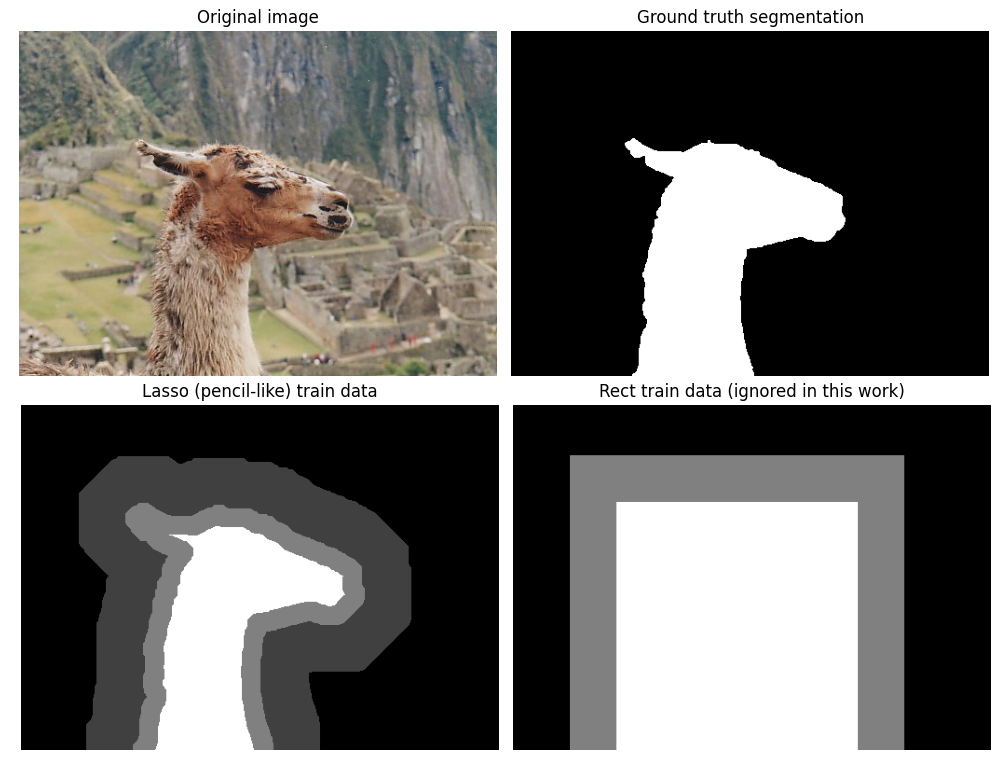
\includegraphics[scale=0.21]{figuras/grabcut-dataset}
    \source{\fonteautor}
  \end{figure}

\end{frame}

\begin{frame}{Anotação lasso no dataset GrabCut}

  \begin{columns}{}

    % tabela com descrição da anotação
    \begin{column}{0.62\textwidth}
      \begin{table}[!h]\label{tab:grabcut-label}
        \centering
          \resizebox{\columnwidth}{!}{%
          \begin{tabular}{lc}
            \toprule
            Descrição                             & Nível de cinza \\
            \midrule \midrule
            fundo                                 & 0              \\
            fundo [\textbf{treinamento}]          & 64             \\
            região de inferência                  & 128            \\
            primeiro plano [\textbf{treinamento}] & 255            \\
            \bottomrule
          \end{tabular}}
        \source{\cite{rother2004grabcut}}
      \end{table}
    \end{column}

    % imagem de exemplo
    \begin{column}{0.6\textwidth}
      \begin{figure}\label{fig:grabcut-dataset-lasso}
        \centering
        
\includegraphics[scale=0.35]{figuras/grabcut-dataset-lasso}
        \source{\cite{rother2004grabcut}}
      \end{figure}
    \end{column}

  \end{columns}
\end{frame}

\subsection{Métodos de referência}
\begin{frame}{Métodos de referência}

No artigo~\cite{wang2023review}, os autores realizam uma revisão de
sete métodos de segmentação interativa baseados em grafos. Esses
métodos são avaliados utilizando o dataset GrabCut, entre outros.

\begin{enumerate}
    \item GrabCut
    \item LazySnapping
    \item OneCut
    \item Saliency Cuts
    \item Iterated Graph Cuts
    \item DenseCut
    \item Deep GrabCut
\end{enumerate}

\end{frame}

\subsection{Métricas de avaliação}
\begin{frame}{Métricas de avaliação}
  As métricas de avaliação que este trabalho será submetido são:


  \begin{equation*}\label{eq:metricas}
    \begin{aligned}
      Precision &= \dfrac{TP}{TP + FP} \\~\\
      Recall &= \dfrac{TP}{TP + FN} \\~\\
      F1 &= \dfrac{2 \cdot Precision \cdot Recall}{Precision + Recall} \\~\\
      IoU &= \dfrac{\left| A \cap B \right|}{\left| A \cup B \right|}
    \end{aligned}
  \end{equation*}

\end{frame}


\section{Resultados}

\begin{frame}{Avaliação qualitativa}
  \begin{figure}\label{fig:imagens-avaliadas}
    \centering
    \caption{16 imagens do dataset GrabCut usadas na avaliação qualitativa.}
    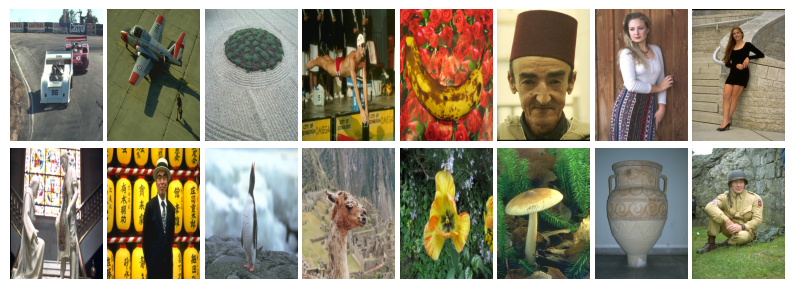
\includegraphics[scale=0.55]{figuras/imagens-avaliadas}
    \source{Elaborado pelo autor baseado no dataset GrabCut~\cite{rother2004grabcut}}
  \end{figure}
\end{frame}


\subsection{Resultados qualitativos}
\begin{frame}{Avaliação qualitativa: métodos de referência}
    \begin{figure}\label{fig:grabcut-comparacao-split1}
    \centering
    \caption{Avaliação qualitativa de métodos de referência no dataset GrabCut.}
    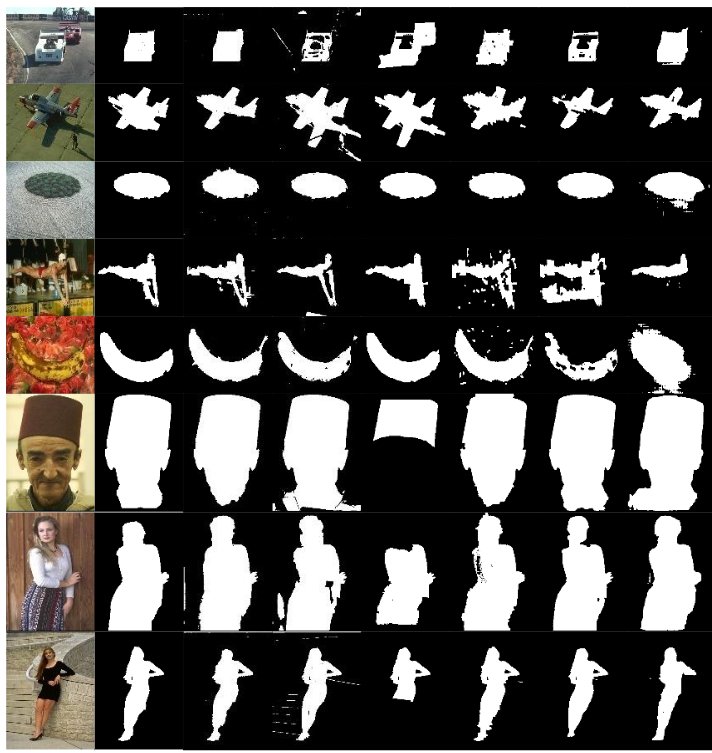
\includegraphics[scale=0.325]{figuras/grabcut-comparacao-split1}
    \source{\cite{wang2023review}}
  \end{figure}
\end{frame}

\begin{frame}{Avaliação qualitativa: métodos de referência}
  \begin{figure}\label{fig:grabcut-comparacao-split2}
    \centering
    \caption{Avaliação qualitativa de métodos de referência no dataset GrabCut.}
    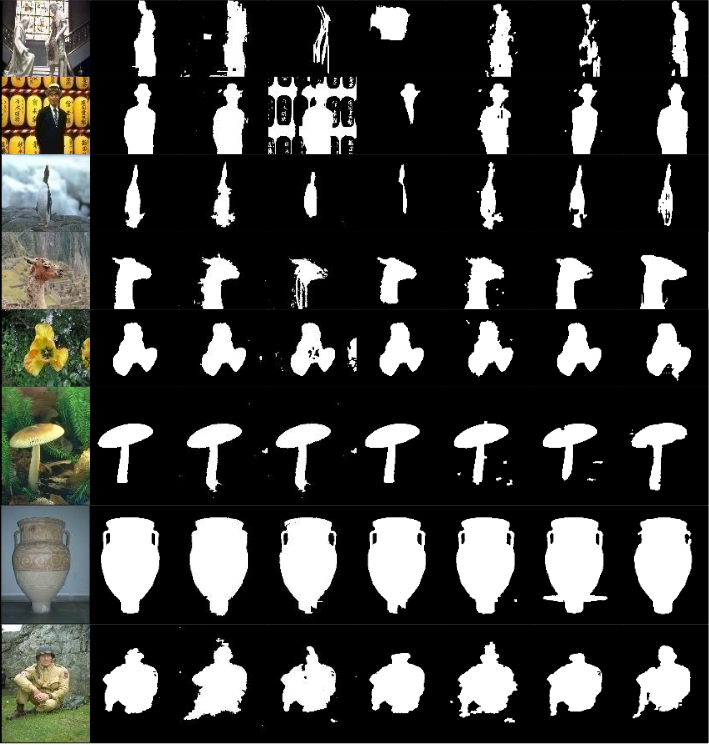
\includegraphics[scale=0.325]{figuras/grabcut-comparacao-split2}
    \source{\cite{wang2023review}}
  \end{figure}
\end{frame}

\begin{frame}{Avaliação qualitativa: método EGSIS}
  \begin{figure}\label{fig:egsis-qualitativa}
    \centering
    \caption{Avaliação qualitativa do método EGSIS no dataset GrabCut.}
    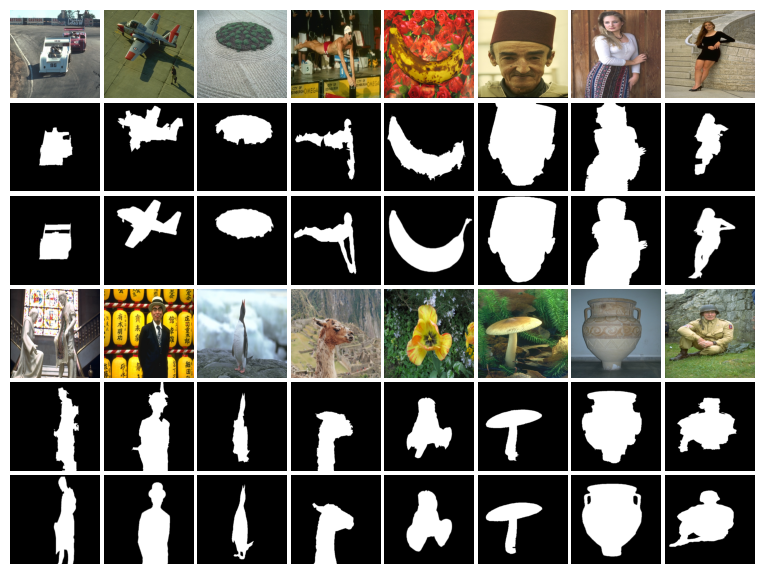
\includegraphics[scale=0.43]{figuras/egsis-qualitativa-transposto}
    \source{Elaborado pelo autor.}
  \end{figure}
\end{frame}

\begin{frame}{Avaliação qualitativa: melhor resultado}
  \begin{figure}\label{fig:egsis-melhor}
    \centering
    \caption{Melhor resultado do método EGSIS entre as 16 imagens.}
    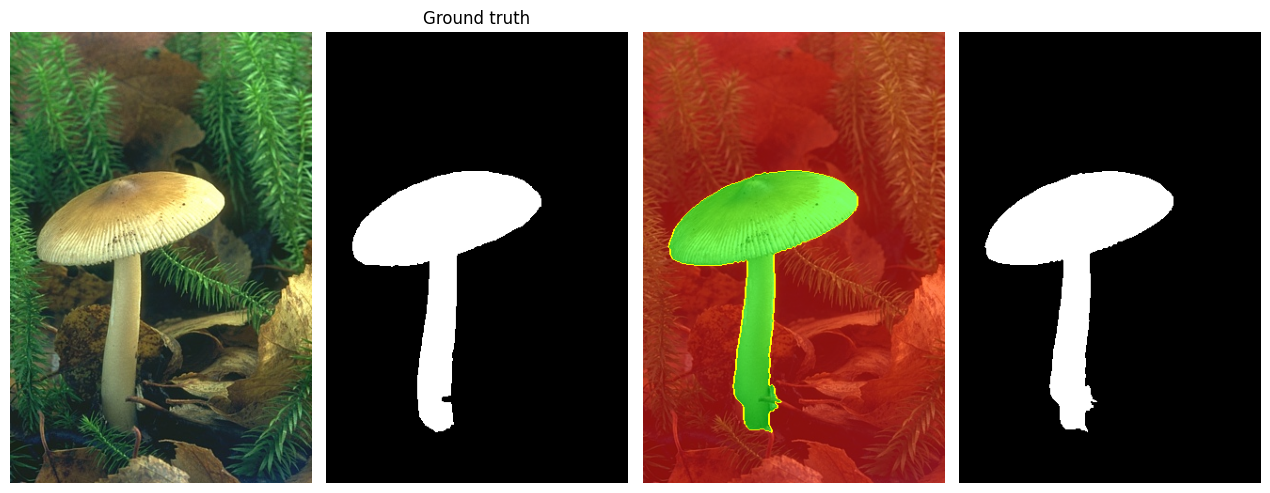
\includegraphics[scale=0.35]{figuras/egsis-melhor}
    \source{Elaborado pelo autor.}
  \end{figure}
\end{frame}

\begin{frame}{Avaliação qualitativa: pior resultado}
  \begin{figure}\label{fig:egsis-pior}
    \centering
    \caption{Pior resultado do método EGSIS entre as 16 imagens.}
    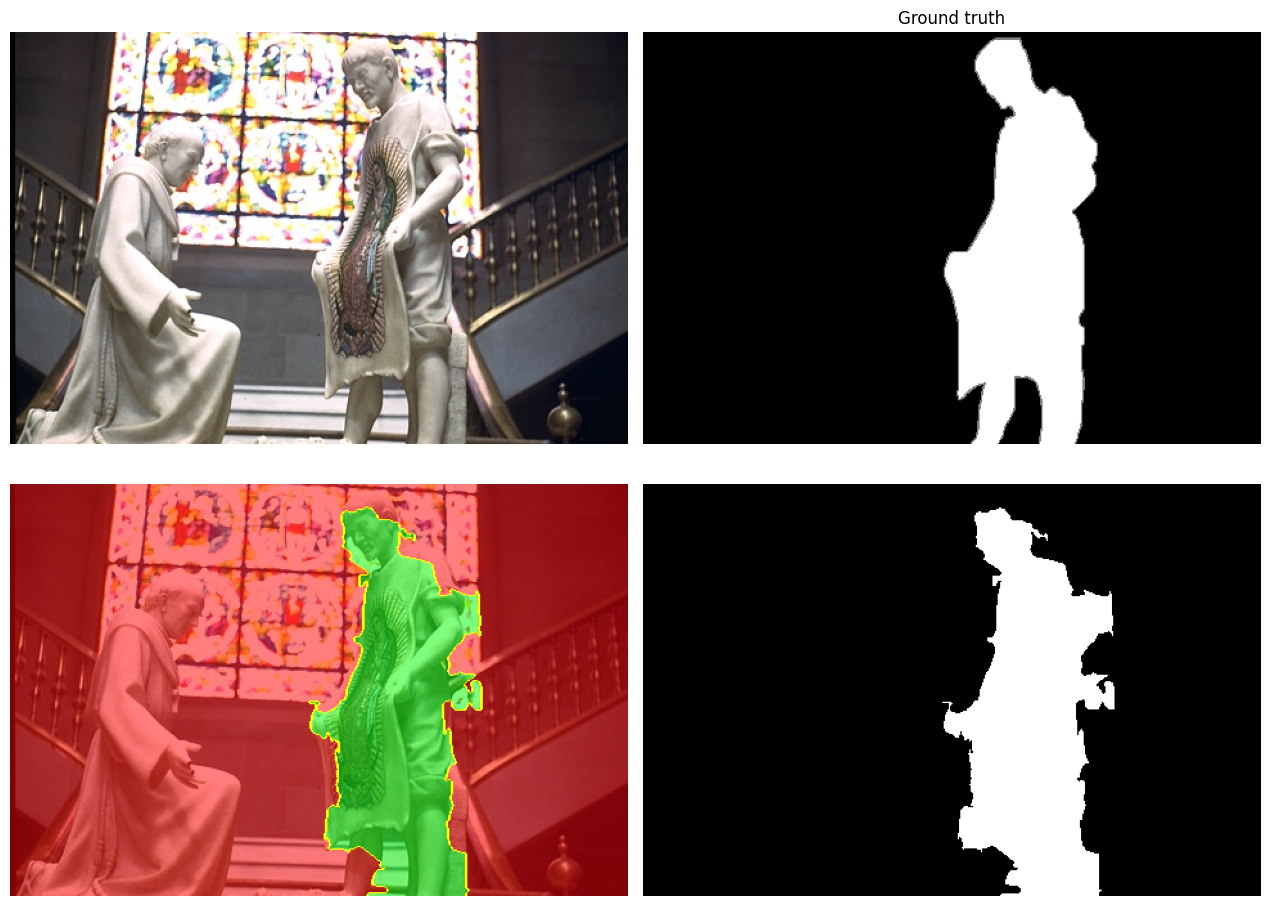
\includegraphics[scale=0.36]{figuras/egsis-pior}
    \source{Elaborado pelo autor.}
  \end{figure}
\end{frame}


\subsection{Variação na quantidade de superpixels}
\begin{frame}{Variação na quantidade de superpixels}
  \begin{table}[!h]
    \centering
    \caption{Resultados dos experimentos ao variar o número de superpixels e o método de extração
      de características. Em negrito os melhores resultados.}\label{tab:variacao-superpixels}
    \resizebox{\columnwidth}{!}{%
    \begin{tabular}{lcccc}
      \toprule
      \textbf{Método}            & \textbf{Recall} & \textbf{Precision} & \textbf{F1}     & \textbf{IoU}    \\
      \midrule \midrule
      $EGSIS(s=50, f=gabor)$     & 0.7882          & 0.9225             & 0.8414          & 0.7412          \\
      $EGSIS(s=100, f=gabor)$    & 0.8592          & 0.9505             & 0.8992          & 0.8232          \\
      $EGSIS(s=150, f=gabor)$    & 0.8691          & 0.9550             & 0.9066          & 0.8354          \\
      $EGSIS(s=200, f=gabor)$    & 0.8799          & \textbf{0.9620}    & 0.9167          & 0.8511          \\
      $EGSIS(s=50, f=comatrix)$  & 0.7882          & 0.9225             & 0.8414          & 0.7412          \\
      $EGSIS(s=100, f=comatrix)$ & 0.8617          & 0.9510             & 0.9010          & 0.8259          \\
      $EGSIS(s=150, f=comatrix)$ & 0.8777          & 0.9552             & 0.9125          & 0.8441          \\
      $EGSIS(s=200, f=comatrix)$ & \textbf{0.8877} & 0.9611             & \textbf{0.9212} & \textbf{0.8578} \\
      \bottomrule
    \end{tabular}
    }
    \source{\fonteautor}
  \end{table}
\end{frame}

\subsection{Resultados quantitativos}
\begin{frame}{Resultados quantitativos}
  \begin{table}[!h]
    \centering
    \caption{Resultados
      comparativos entre o método EGSIS e métodos estado-da-arte para
      segmentação interativa baseado em grafos. Em negrito os melhores
      resultados, em vermelho os piores.}\label{tab:resultados-estado-da-arte}
    \resizebox{\columnwidth}{!}{%
      \begin{tabular}{lcccc}
        \toprule
        \textbf{Método}            & \textbf{Recall} & \textbf{Precision} & \textbf{F1}     & \textbf{IoU}    \\
        \midrule \midrule
        GrabCut                    & 0.9668          & 0.9213             & \textbf{0.9407} & \textbf{0.8927} \\
        LazySnapping               & \textbf{0.9681} & 0.9104             & 0.9357          & 0.8842          \\
        OneCut                     & 0.8585          & \red{0.7926}       & \red{0.7899}    & \red{0.6974}    \\
        Saliency Cuts              & \red{0.8371}    & 0.8892             & 0.8255          & 0.7458          \\
        Iterated Graph Cuts        & 0.9614          & 0.8878             & 0.9212          & 0.8597          \\
        DenseCut                   & 0.8427          & 0.9418             & 0.8561          & 0.7927          \\
        Deep GrabCut               & 0.8854          & 0.8774             & 0.8701          & 0.7849          \\
        $EGSIS(s=200, f=gabor)$    & 0.8799          & \textbf{0.9620}    & 0.9167          & 0.8511          \\
        $EGSIS(s=200, f=comatrix)$ & 0.8877          & 0.9611             & 0.9212          & 0.8578          \\
        \bottomrule
      \end{tabular}
    }
    \source{Baseado nos resultados encontrados no artigo~\cite{wang2023review}}
  \end{table}
\end{frame}


\section{Conclusão}
\begin{frame}{Principais conclusões}
  \begin{enumerate}[<+->]

  \item Desenvolvimento de um novo algoritmo chamado EGSIS que permite
    a resolução de problemas de segmentação interativa de imagens.

  \item O algoritmo EGSIS apresentou uma \textbf{eficácia equiparável}
    aos métodos estado-da-arte baseados em grafos para segmentação
    interativa de imagens.

  \item A qualidade da segmentação final é altamente dependente da
    qualidade da pré-segmentação com superpixels.

  \item Melhores resultados foram alcançados com um \textbf{maior número de
    superpixels}, mas isso também aumentou o tempo de execução do
    algoritmo.

  \item O algoritmo possui várias partes móveis e trocáveis, permitindo a
    evolução de técnicas para melhorar a qualidade de segmentação final.

  \end{enumerate}
\end{frame}

\subsection{Limitações e desafios}
\begin{frame}{Limitações e desafios}
  \begin{enumerate}[<+->]
  \item A busca por trabalhos de referência com a palavra-chave
    semi-supervisionado foi desafiadora, mas a mudança para
    \textbf{segmentação transdutiva e interativa} permitiu encontrar trabalhos
    mais relevantes.

  \item A falta de datasets para segmentação interativa com anotação
    parcial inicial limitou a exploração e comparação com outros
    datasets e técnicas, restringindo o trabalho ao dataset GrabCut.

  \item O algoritmo EGSIS permite segmentação interativa
    multi-classes, mas a dificuldade em encontrar datasets públicos com rotulações
    parciais restringiu o avanço desta linha de pesquisa.

  \item Há espaço para crescimento na pesquisa de algoritmos de
    segmentação interativa multi-classes. Um novo conjunto de dados para
    benchmark seria uma contribuição relevante.

  \end{enumerate}
\end{frame}


\subsection{Trabalhos futuros}
\begin{frame}{Trabalhos futuros}
  \begin{enumerate}[<+->]
  \item A pesquisa sobre algoritmos transdutivos de segmentação de
imagens ainda está em evolução, mas com menos volume que as técnicas
indutivas.

  \item Métodos de superpixel, extração de características, construção
da rede complexa e dinâmica coletiva são partes móveis que podem ser
refinadas.

  \item Extração de características de imagens: este trabalho
limitou-se à matrizes de co-ocorrências e filtros de Gabor. Trabalhos
futuros podem explorar \textbf{técnicas estado-da-arte de extração de
características}.

\item \textbf{Minimização do número de cliques de anotação}: estudos recentes~\cite{chen2022focalclick}
  buscam técnicas que minimizem o número de cliques de anotação
  necessários para alcançar segmentações de boa qualidade.


  \end{enumerate}
\end{frame}


%% ---------------------------------------------------------------------------
% Slides de referência
\section{Referências}
\begin{frame}[t, allowframebreaks]
  \frametitle{Referências}
  % Inserting the references file
  \bibliography{3-pos-textuais/referencias.bib}

\end{frame}

%% ---------------------------------------------------------------------------
% Slide final com agradecimento e contato
\begin{frame}{}
    \centering
    \huge{\textbf{\example{Obrigado pela atenção!}}}

    \vspace{1cm}

    \Large{\textbf{Contato:}}
    \newline
    \vspace*{0.5cm}
    \large{\email{manoel.machado@alu.ufc.br}}
\end{frame}

\end{document}
